\documentclass[utf8x]{beamer}

\usepackage[absolute,overlay]{textpos}
\usepackage{amsmath}
\usepackage{amssymb}
\usepackage{animate}
\usepackage{beamerthemesplit}
\usepackage{calc}
\usepackage{clrscode}
\usepackage{fancyvrb}
\usepackage{graphicx}
\usepackage{hyperref}
\usepackage{pgf,tikz}
\usepackage{setspace}
\usepackage{url}
\usepackage{verbatim}
\usetikzlibrary{arrows}

\DeclareGraphicsExtensions{.pdf,.png,.jpg}


\newcounter{lines per second}
\newcounter{lines per page}
\newcounter{frames per second}
\newcounter{total frames}
\newcounter{total lines}
\newcommand{\verbfilename}{}
\newsavebox{\verbbox}
\newlength{\verbtotalheight}
\expandafter\newlength\csname verb max offset\endcsname
\newlength{\verboffsetperframe}
\newcounter{total time}

\newcommand{\putat}[3]{\begin{picture}(0,0)(0,0)\put(#1,#2){#3}\end{picture}}

% \scrollfile[adjustment]{file name}{total time}{fps}
\newcommand{\scrollfile}[4][-0.5\textheight]{
  \setcounter{total time}{#3}
  \setcounter{frames per second}{#4}
  \renewcommand{\verbfilename}{#2}
  \savebox{\verbbox}{\tiny\fvset{fontsize=\tiny}\BVerbatimInput{\verbfilename}}
  \setlength{\verbtotalheight}{\totalheightof{\usebox{\verbbox}}}
  \setcounter{total frames}{\value{frames per second} * \value{total time}}
  \expandafter\setlength\expandafter{\csname verb max offset\endcsname}{\verbtotalheight + #1}
  \setlength{\verboffsetperframe}{\csname verb max offset\endcsname / \value{total frames}}
  \hspace*{-1cm}
  \begin{animateinline}[autoplay]{\the\value{frames per second}}
    \multiframe{\value{total frames}}{
      dOffset=-1cm+\the\verboffsetperframe
    }{%
    \raisebox{\dOffset}[\height][\depth]{\usebox{\verbbox}}%
  }
\end{animateinline}
}

\pdfinfo {
  /Title (Casting Spells)
  /Subject (Casting Spells in Magic: the Gathering)
  /Author () 
  /Keywords (Magic, Gathering, Cast, Spells, Comprehensive, Rules, 601)
}

\begin{document}
  
\title{Casting Spells}
\date{September 6, 2014}
\author{Bobby Fortanely}

\begin{frame}
  \titlepage
\end{frame}
  
\section*{Outline}
  \begin{frame}{Outline}
    \tableofcontents
  \end{frame}
\section{What is a spell?}
  \subsection*{}
  
    \begin{frame}{What is a spell?}
      \begin{itemize}
        \item Spells are cards on the stack
        \item Copies of spells are also spell
      \end{itemize}
      \putat{185}{-30}{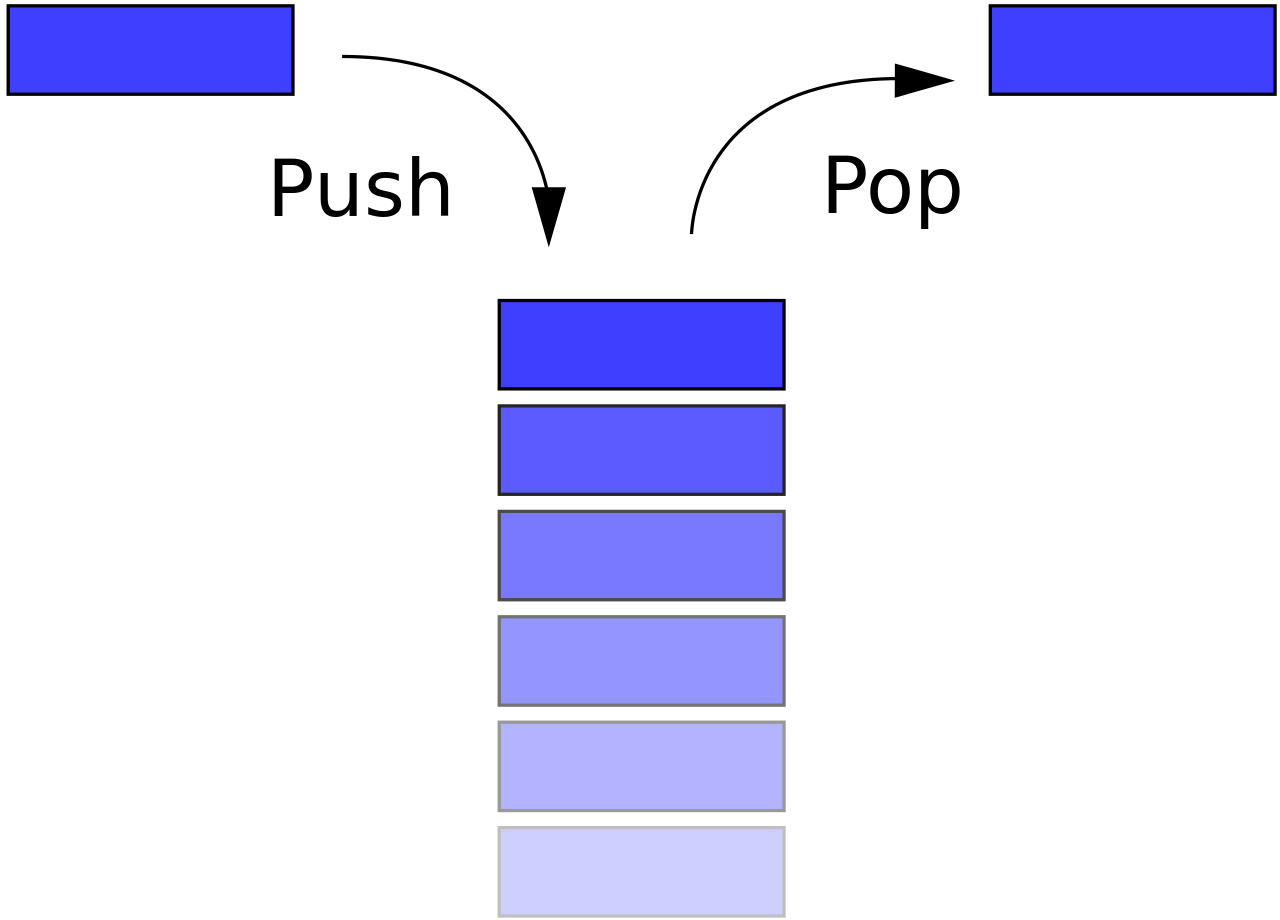
\includegraphics[scale=0.1]{Data_stack}}
      \putat{239}{-30}{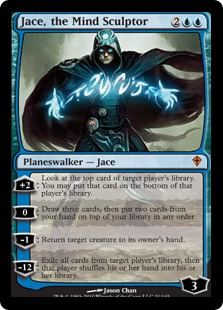
\includegraphics[scale=0.06, angle=90]{JTMS}}
      \putat{235}{-20}{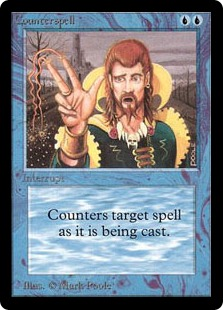
\includegraphics[scale=0.06, angle=90]{Counterspell}}
      \putat{231}{-10}{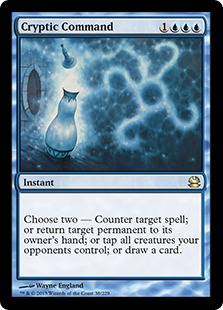
\includegraphics[scale=0.06, angle=90]{CrypticCommand}}
      \putat{228}{1}{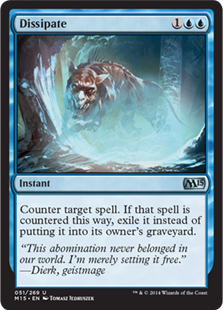
\includegraphics[scale=0.05, angle=90]{Dissipate}}
      \putat{225}{11}{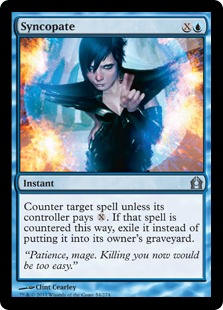
\includegraphics[scale=0.06, angle=90]{Syncopate}}
      \putat{221}{22}{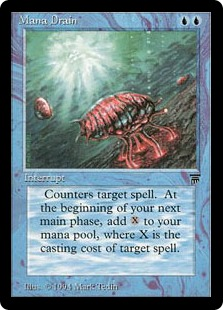
\includegraphics[scale=0.06, angle=90]{ManaDrain}}
    \end{frame}

    \begin{frame}{What can be a spell}
      \begin{itemize}
        \item Artifact 
      \only<1>{\putat{100}{-100}{
        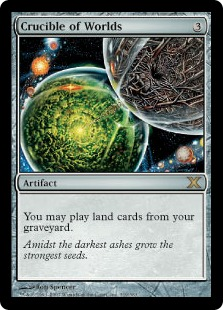
\includegraphics[scale=0.5]{CrucibleofWorlds}}}
      \pause
        \item Creature 
      \only<2>{\putat{95}{-84}{
        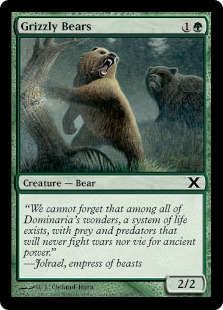
\includegraphics[scale=0.5]{GrizzlyBear}}}
      \pause
        \item Enchantment 
      \only<3>{\putat{72}{-66}{
        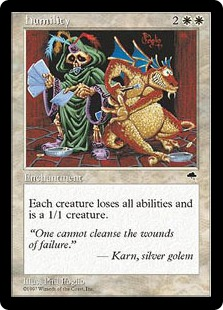
\includegraphics[scale=0.5]{Humility}}}
      \pause
        \item Instant
      \only<4>{\putat{102}{-49}{
        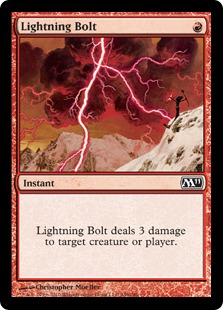
\includegraphics[scale=0.5]{LightningBolt}}}
      \pause
        \item Planeswalker
      \only<5>{\putat{75}{-32}{
        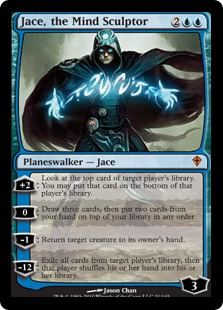
\includegraphics[scale=0.5]{JTMS}}}
      \pause
        \item Sorcery
      \only<6>{\putat{100}{-15}{
        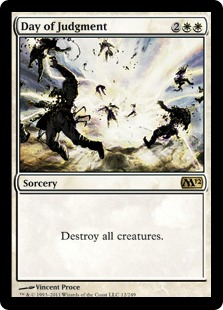
\includegraphics[scale=0.5]{Day}}}
      \end{itemize}
    \end{frame}

    \begin{frame}{What can not be a spell}
      \begin{itemize}
        \item LAND
      \only<1>{\putat{97}{-100}{
        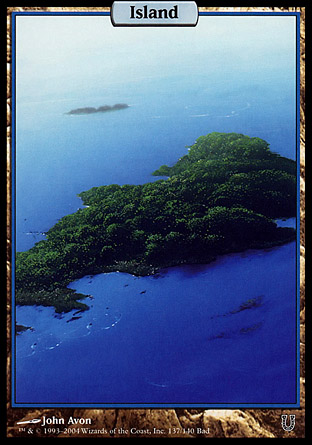
\includegraphics[scale=1.1]{Island}}}
      \pause
      \only<2>{\putat{94}{-99}{
        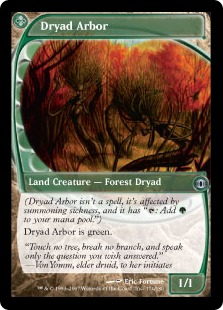
\includegraphics[scale=.5]{DryadArbor}}}
      \pause
        \item Conspiracy
      \only<3>{\putat{84}{-83}{
        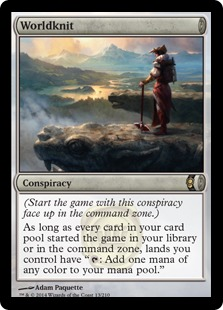
\includegraphics[scale=.5]{Worldknit}}}
      \pause
        \item Phenomenon
      \only<4>{\putat{35}{-73}{
        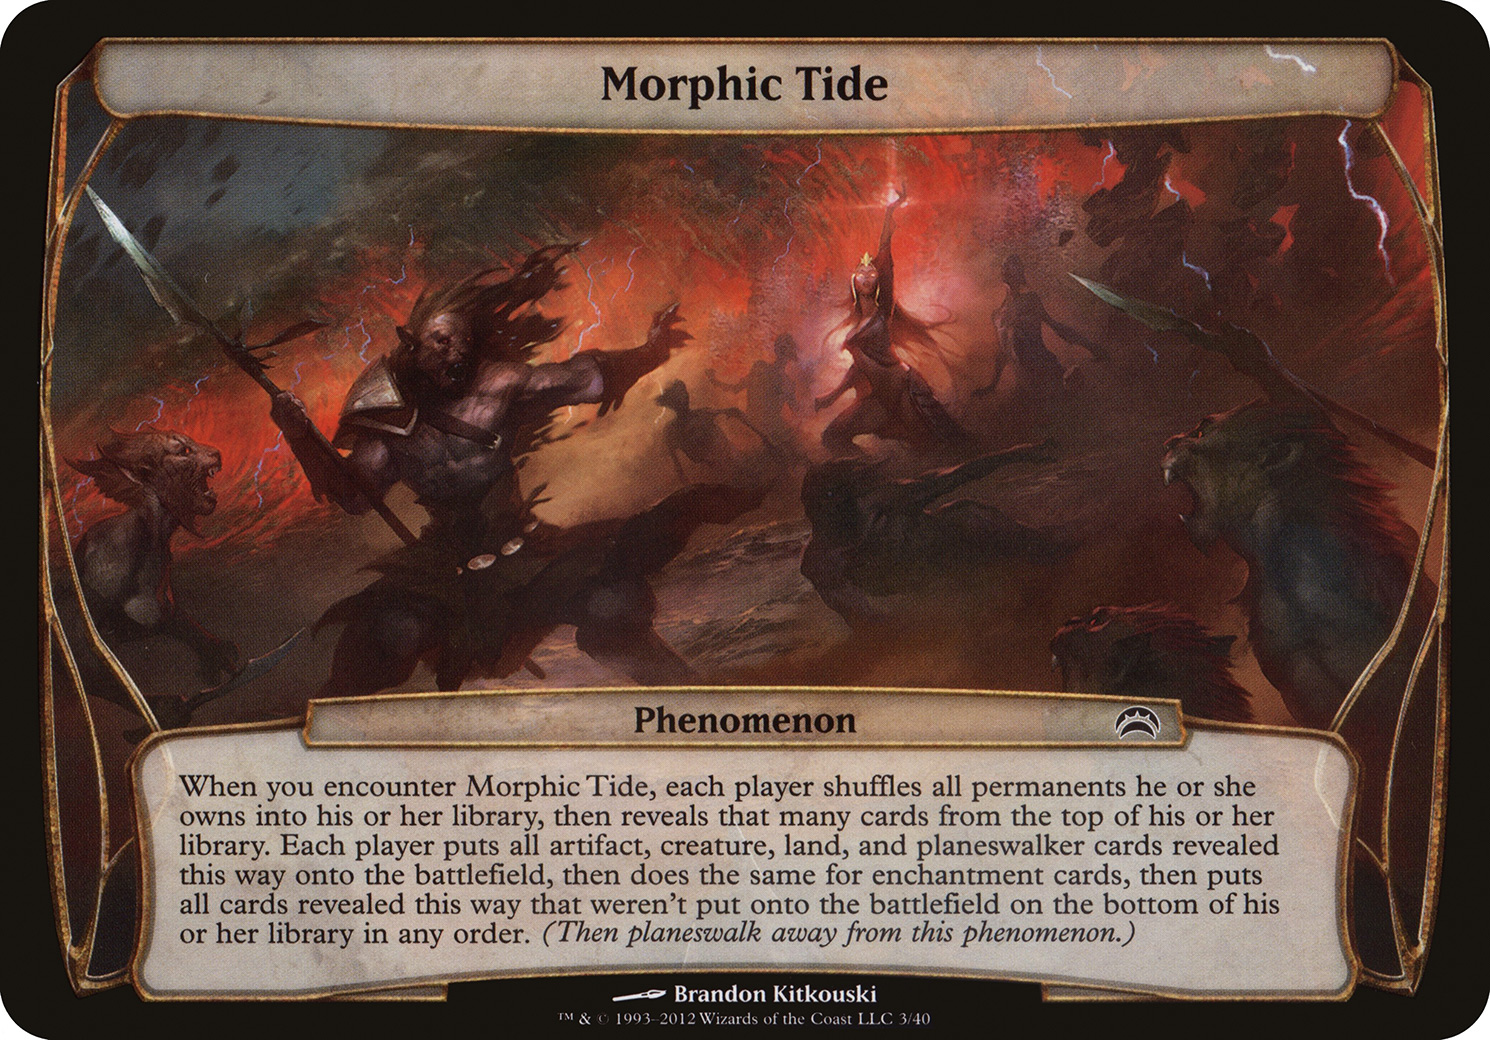
\includegraphics[scale=.5]{MorphicTide}}}
      \pause
        \item Plane
      \only<5>{\putat{68}{-55}{
        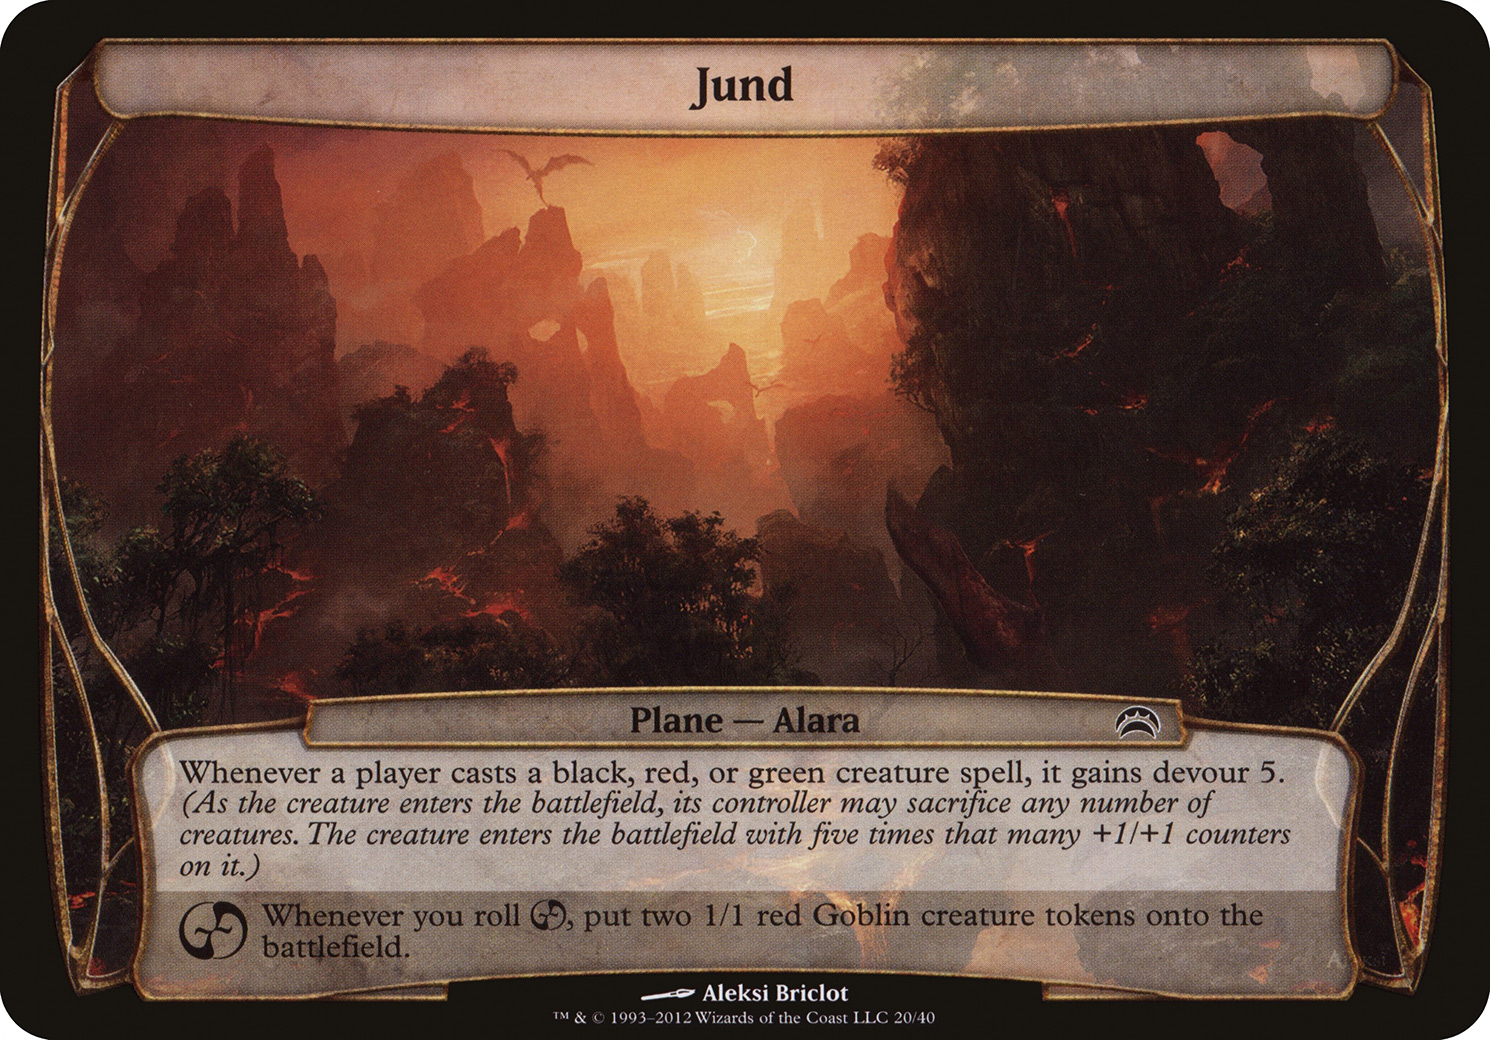
\includegraphics[scale=.5]{Jund}}}
      \pause
        \item Scheme
      \only<6-7>{\putat{88}{-35}{
        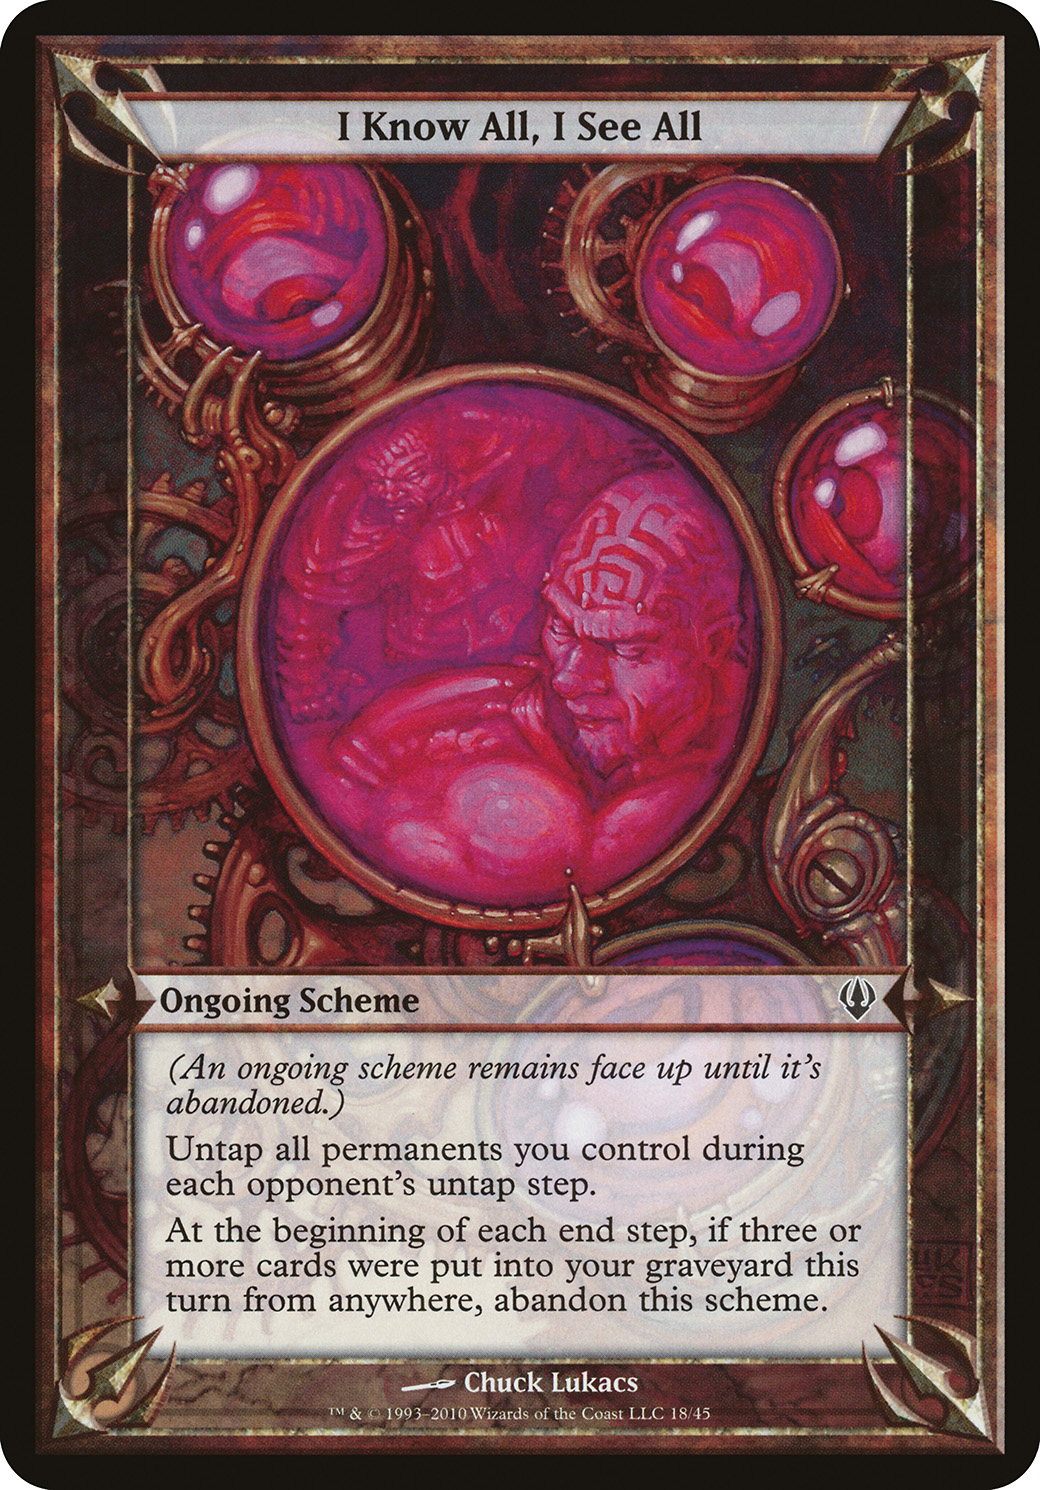
\includegraphics[scale=.8]{IKnowAll}}}
      \pause
        \item Vanguard
      \only<7>{\putat{78}{-18}{
        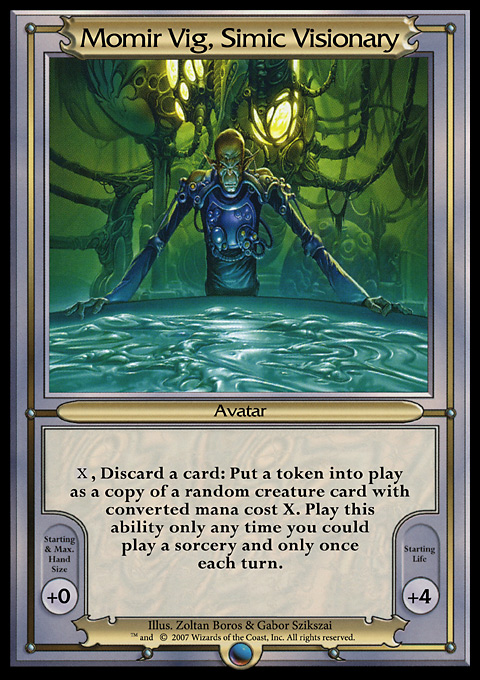
\includegraphics[scale=.21]{Momir}}}
      \end{itemize}
    \end{frame}

\section{Steps of Casting a spell}
  \subsection*{Steps of Casting a Spell}
  
    \begin{frame}{Steps of Casting a Spell}
      \begin{itemize}
        \item Announce Spell
        \item Choices
        \item Targets
        \item Distribute
        \item Determine Cost
        \item Mana Abilities
        \item Payment
      \end{itemize}
    \end{frame}

  \subsection*{Announce Spell}
    \begin{frame}{Announce Spell}
      \putat{105}{-80}{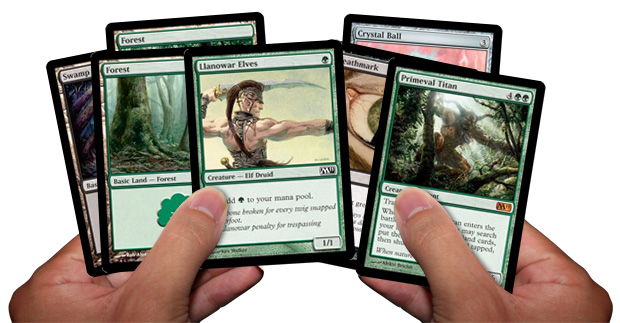
\includegraphics[scale=0.1]{Hand}}
      \putat{185}{-70}{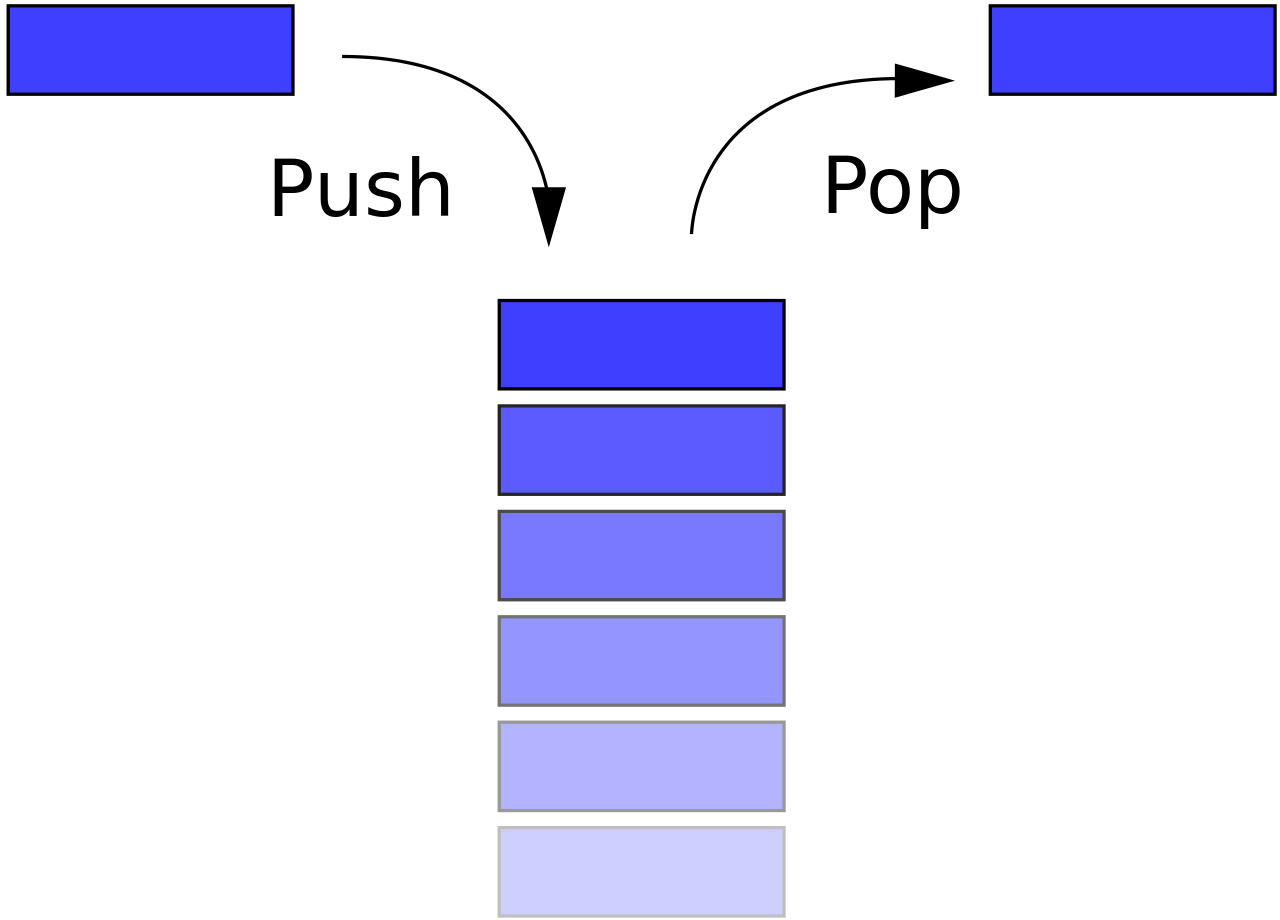
\includegraphics[scale=0.1]{Data_stack}}
      \putat{239}{-70}{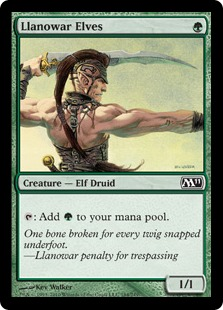
\includegraphics[scale=0.06, angle=90]{LlanowarElves}}
      \begin{itemize}
        \item Announce ``I am casting this spell''
        \item Move to top of stack (usually from hand)
      \end{itemize}
      \begin{textblock*}{100pt}(220pt,218pt)
        $\longrightarrow$
      \end{textblock*}
    \end{frame}

  \subsection*{Choices}
    \begin{frame}{Choices}
      \begin{itemize}
        \item Modes \pause
        \item Splice \pause
        \item Additional Costs \pause
        \item Alternative Costs \pause
        \item Choose X \pause
        \item Hybrid/Phyrexian Mana \pause
      \end{itemize}
    \end{frame}

  \subsection*{Targets}
    \begin{frame}{Targets}
      \begin{itemize}
        \item Choose number of targets, if variable
        \item Must choose all legal target
        \item Target same object once per instance of word ``target''
      \end{itemize}
    \end{frame}

  \subsection*{Distribute}
    \begin{frame}{Distribute}
      \begin{itemize}
        \item Divide/Distribute
        \item At least 1 per target
      \end{itemize}
    \end{frame}

  \subsection*{Determine Cost}
    \begin{frame}{Determine Cost}
      \begin{itemize}
        \item Apply cost additions
        \item Then, apply cost reductions
        \item Finally, apply effects on total costs (Trinisphere)
      \end{itemize}
    \end{frame}

  \subsection*{Mana Abilities}
    \begin{frame}{Mana Abilities}
      \begin{itemize}
        \item Activate mana abilites (only if mana required for payment)
      \end{itemize}
    \end{frame}

  \subsection*{Payment}
    \begin{frame}{Payment}
      Pay costs in any order
    \end{frame}

  \subsection*{Spell is cast}
    \begin{frame}{Payment}
      \begin{itemize}
        \item Spell becomes cast
        \item Trigger trigger
      \end{itemize}
    \end{frame}

 \section{Additional Examples}
  \subsection*{Additional Examples}
  
    \begin{frame}{Additional Examples}
      blah
    \end{frame}
  
\end{document}
  
